% !TeX root = ../dokumentation.tex

\addchap{\langanhang}

\iflang{de}{
	\begin{enumerate}[label=\Alph*.]
		\item Datenquellen
		% \item Tabellen
	\end{enumerate}
}

\pagebreak

\setcounter{section}{0}
\renewcommand{\thesection}{\Alph{section}}
\counterwithin{figure}{section}
\counterwithin{table}{section}
\counterwithin{code}{section}

%\includepdf[pages=-,scale=.9,pagecommand={}]{Aufgabenstellung.pdf} % PDF um 10% verkleinert einbinden --> Kopf- und Fußzeile  werden so korrekt dargestellt. Die Option `pages' ermöglicht es, eine bestimmte Sequenz von Seiten (z.B. 2-10 oder `-' für alle Seiten) auszuwählen.
%\pagebreak

\section{Datenquellen} \label{ch:dataAppendix}

\subsection*{Tweets}

\begin{code}[H]
    \begin{subcode}{0.45\textwidth}
        \small
        Kritischer Austausch bei der Diskussion @co2abgabe. Der CO2-Preis im \#Emissionshandel steigt, das Vertrauen in dieses Instrument muss weiter wachsen! https://t.co/hv1VFPBJrv
        \caption{Beispieltweet von \textit{\_martinneumann}}
    \end{subcode}\hfill
    \begin{subcode}{0.45\textwidth}
        \small
        Treten Sie zurück, Herr Reul! Bin fassungslos, mit welcher Selbstherrlichkeit die NRW-Landesregierung die Profitinteressen von RWE im \#HambacherForst durchsetzt. Der heutige Polizeieinsatz gegen friedliche Sitzblockierer war brutal, selbst Journalisten sind geschlagen worden(1/3) https://t.co/0A3JbnUMmV
        \caption{Beispieltweet von \textit{zdebelhubertus}}
    \end{subcode}\hfill
    \caption[Beispiel -- Tweets]{Beispiel für Tweets von Politikern auf Tweiiter} \label{list:exampleTweets}
\end{code}

\pagebreak

\subsection*{Wahlprogramme} \label{subsec:overviewWP}

% TODO: mit includegraphics einbinden, damit auch caption da ist
\subsubsection*{Beispiel 1: Ausschnitt aus dem Wahlprogramm der CDU zur Bundestagswahl 2017}

\includepdf[pages=32-33,scale=.75,pagecommand={}]{data/examples/party_programs/union_btw17.pdf}

\subsubsection*{Beispiel 2: Ausschnitt aus dem Wahlprogramm der SPD zur Bundestagswahl 2017}

\includepdf[pages=16-17,scale=.75,pagecommand={}]{data/examples/party_programs/spd_btw17.pdf}

\pagebreak

\section{Training} \label{ch:trainingAppendix}

\subsection*{Baseline}

% TODO

\subsection*{fastText}

\begin{figure}[H]
    \begin{subfigure}{0.5\textwidth}
      \centering
      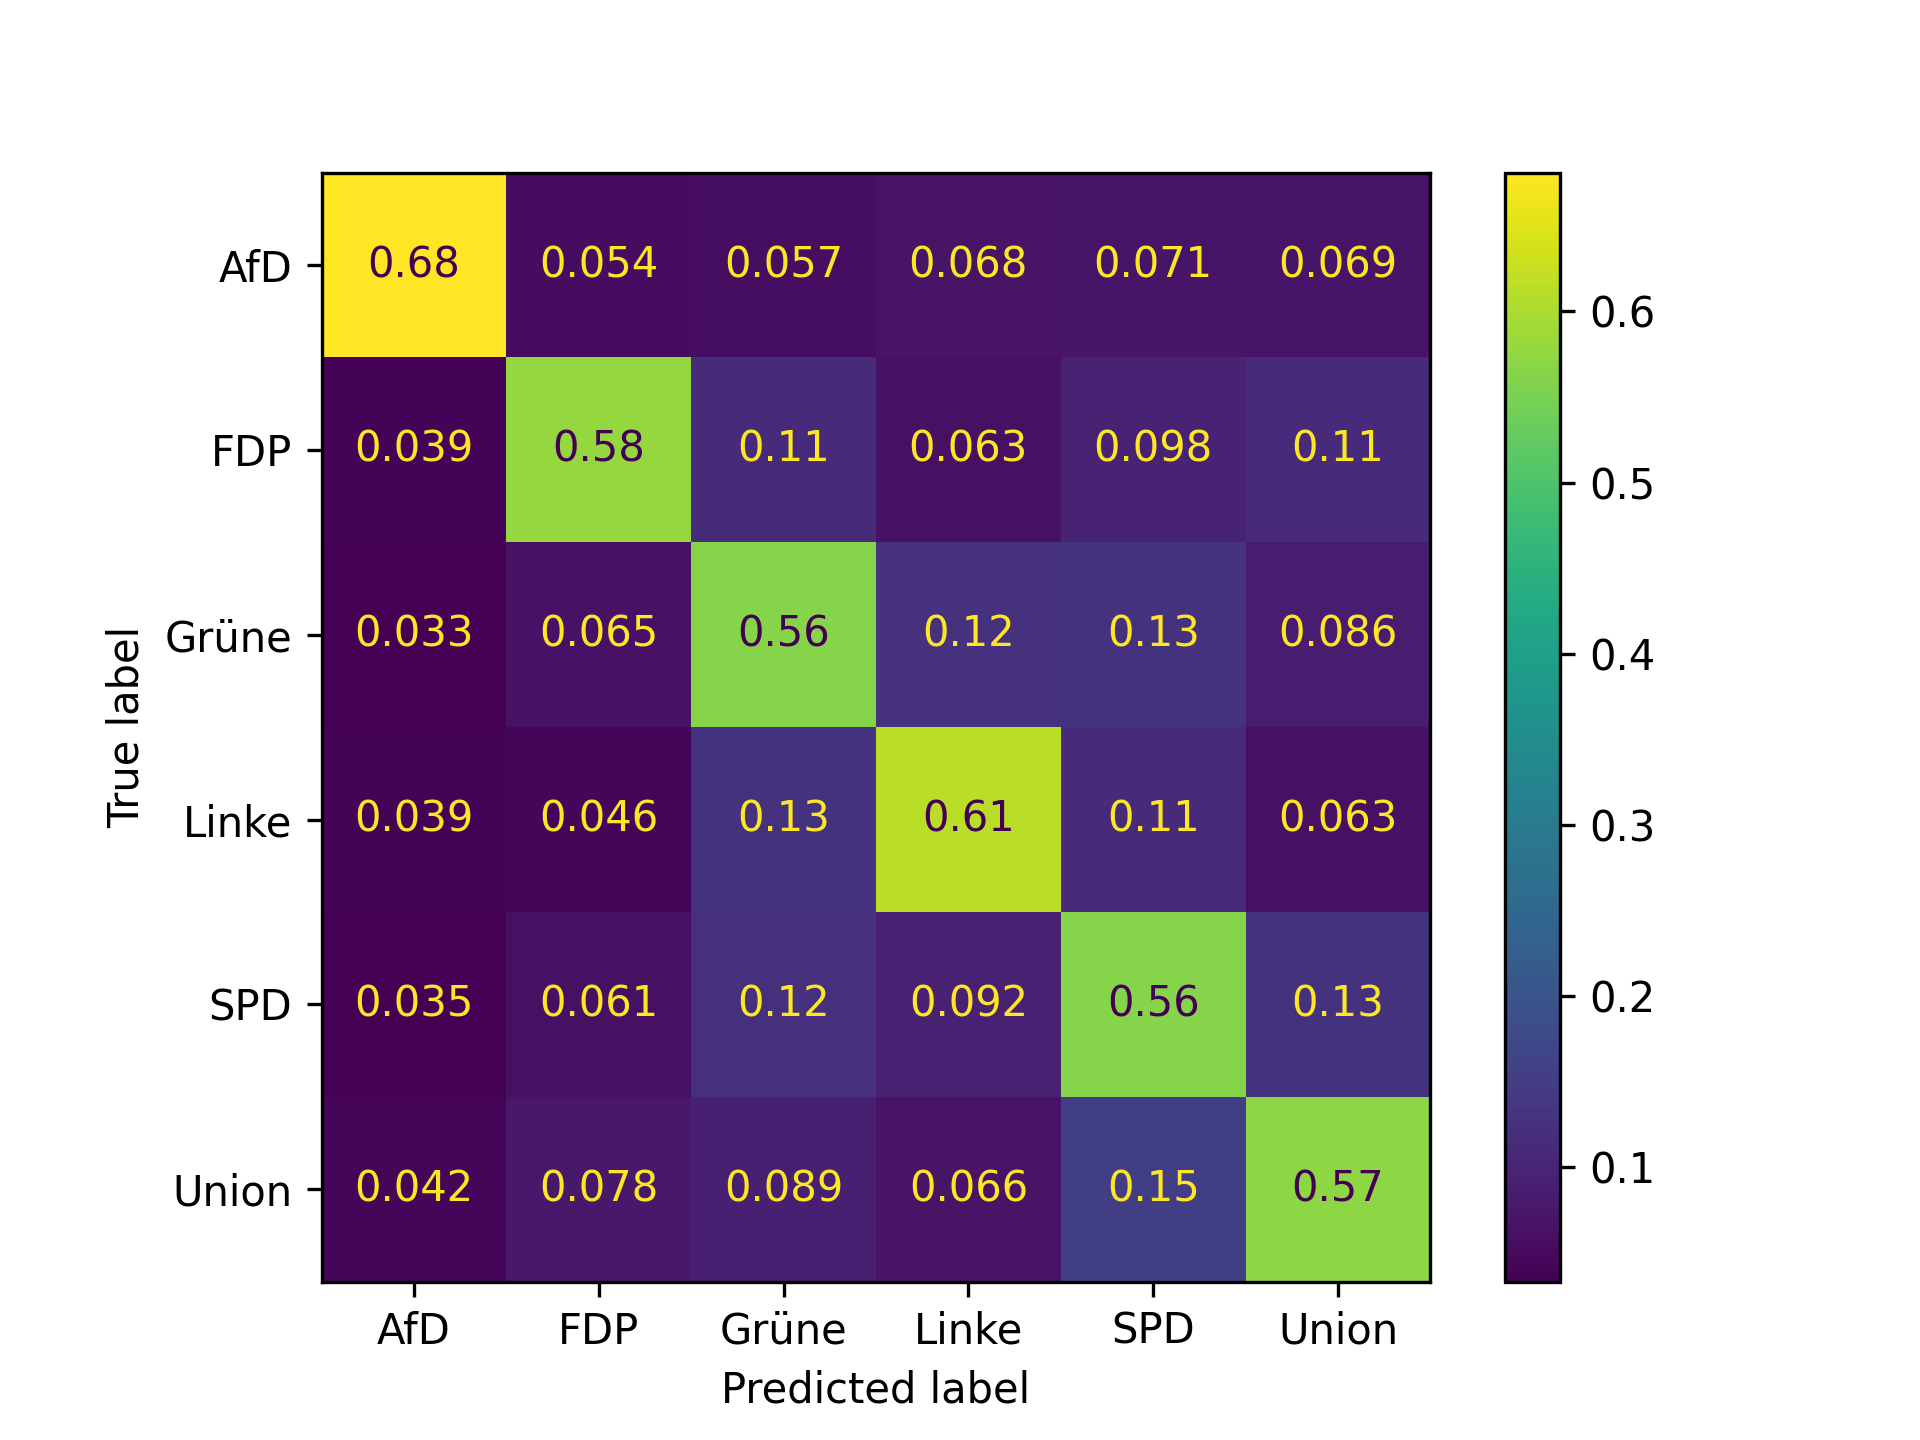
\includegraphics[width=0.9\textwidth]{data/images/modeling/fasttext/none/tweets_confusion_matrix.png}
      \caption{Tweets (\(N = \num{326625}\))} \label{sfig:confusionMatrixFastTextTweetsUnbalanced}
    \end{subfigure}
    \hfill
    \begin{subfigure}{0.5\textwidth}
      \centering
      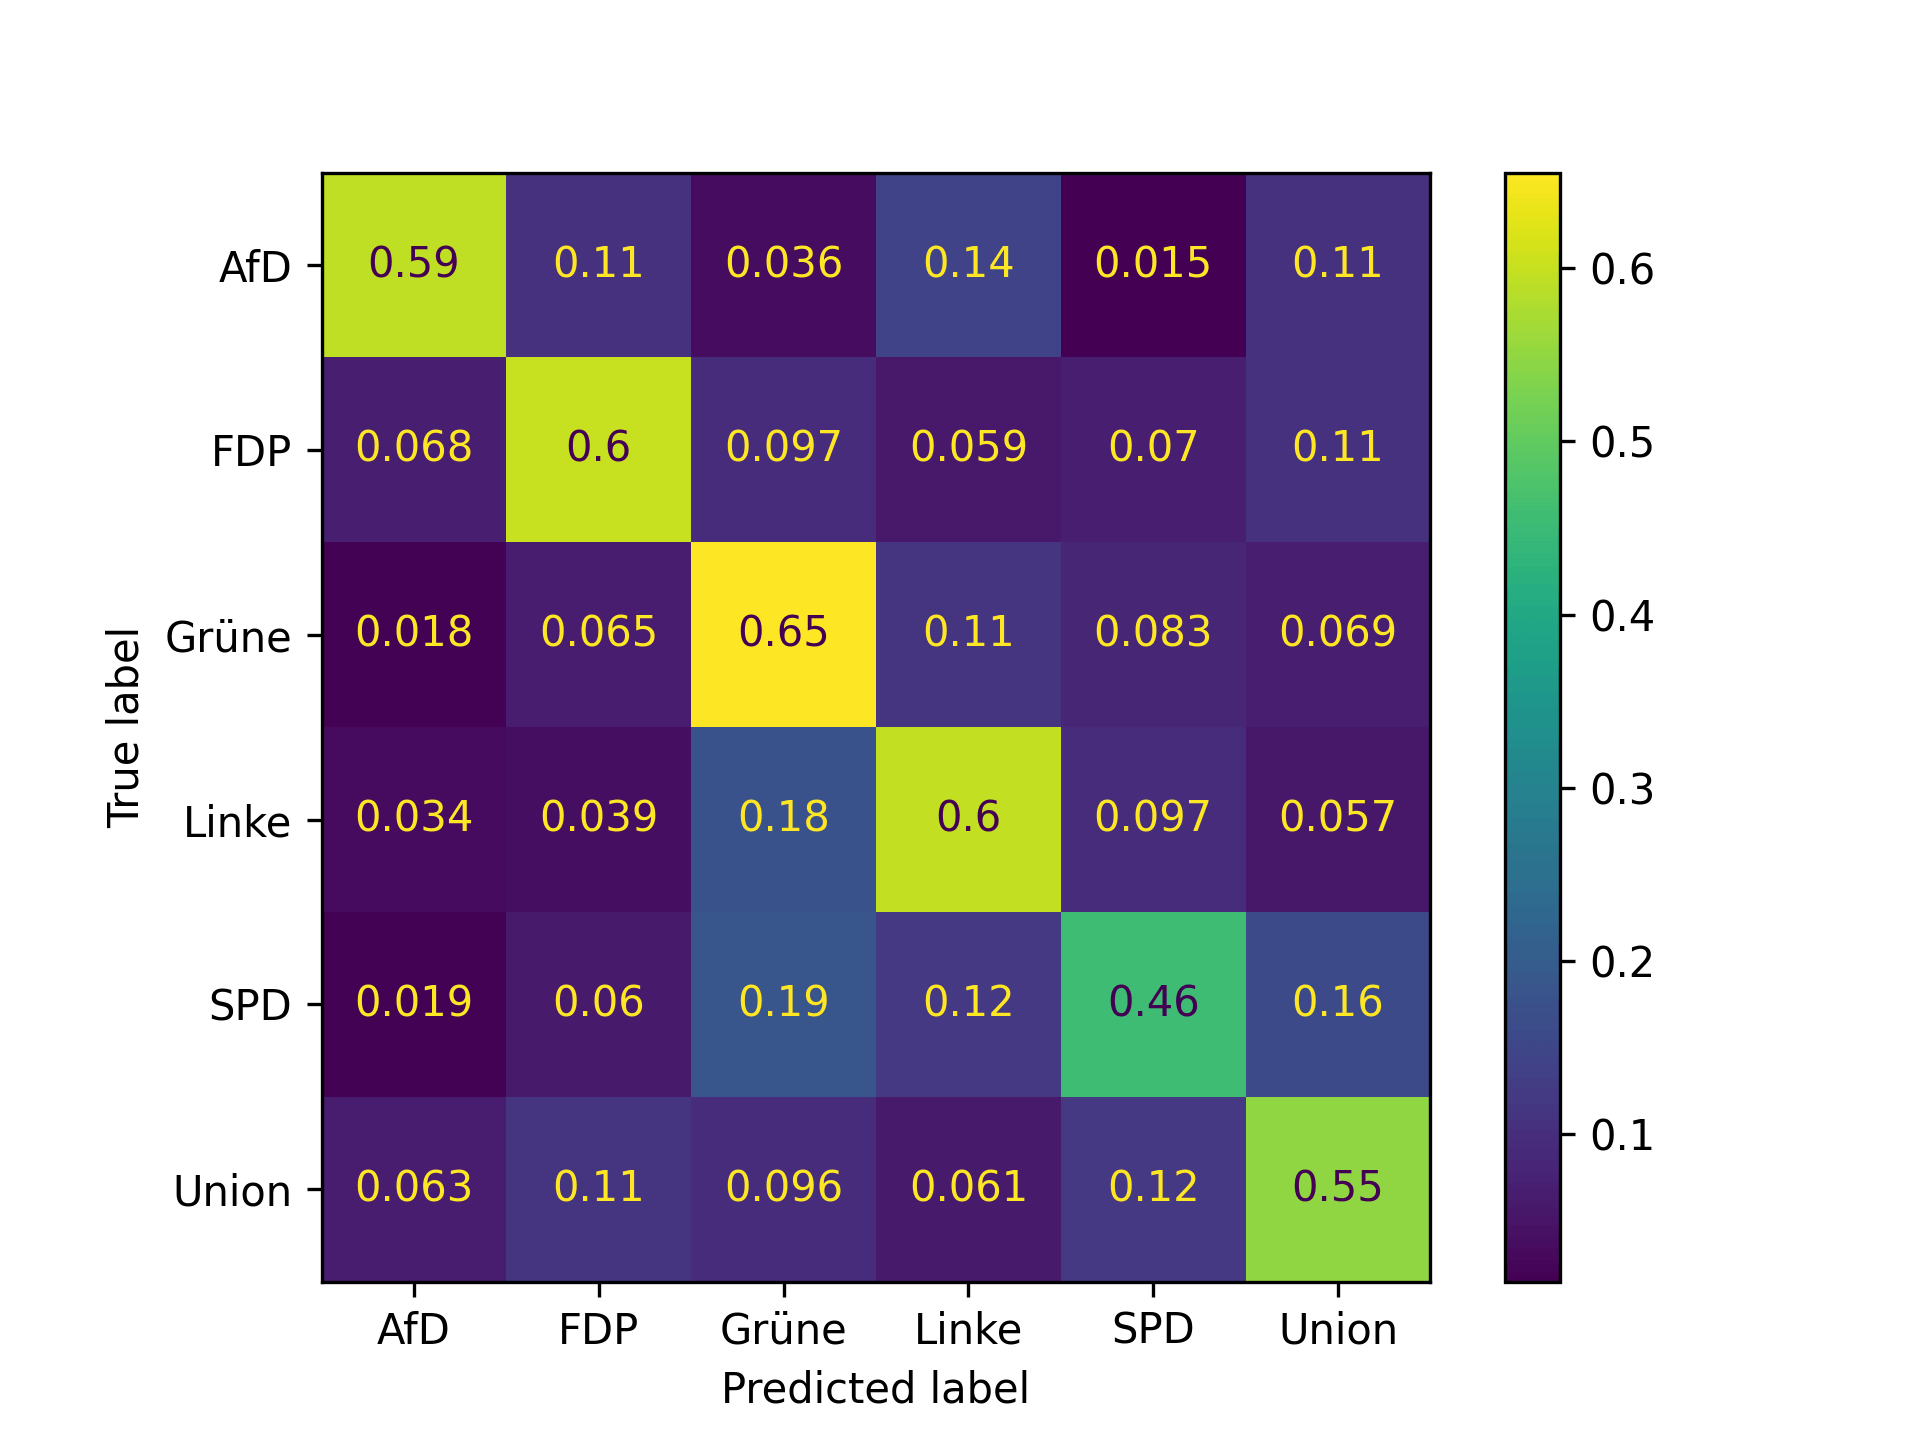
\includegraphics[width=0.9\textwidth]{data/images/modeling/fasttext/none/party_programs_confusion_matrix.png}
      \caption{Wahlprogramme (\(N = \num{27674}\))} \label{sfig:confusionMatrixFastTextManifestUnbalanced}
    \end{subfigure}
    \hfill
    \begin{subfigure}{0.5\textwidth}
      \centering
      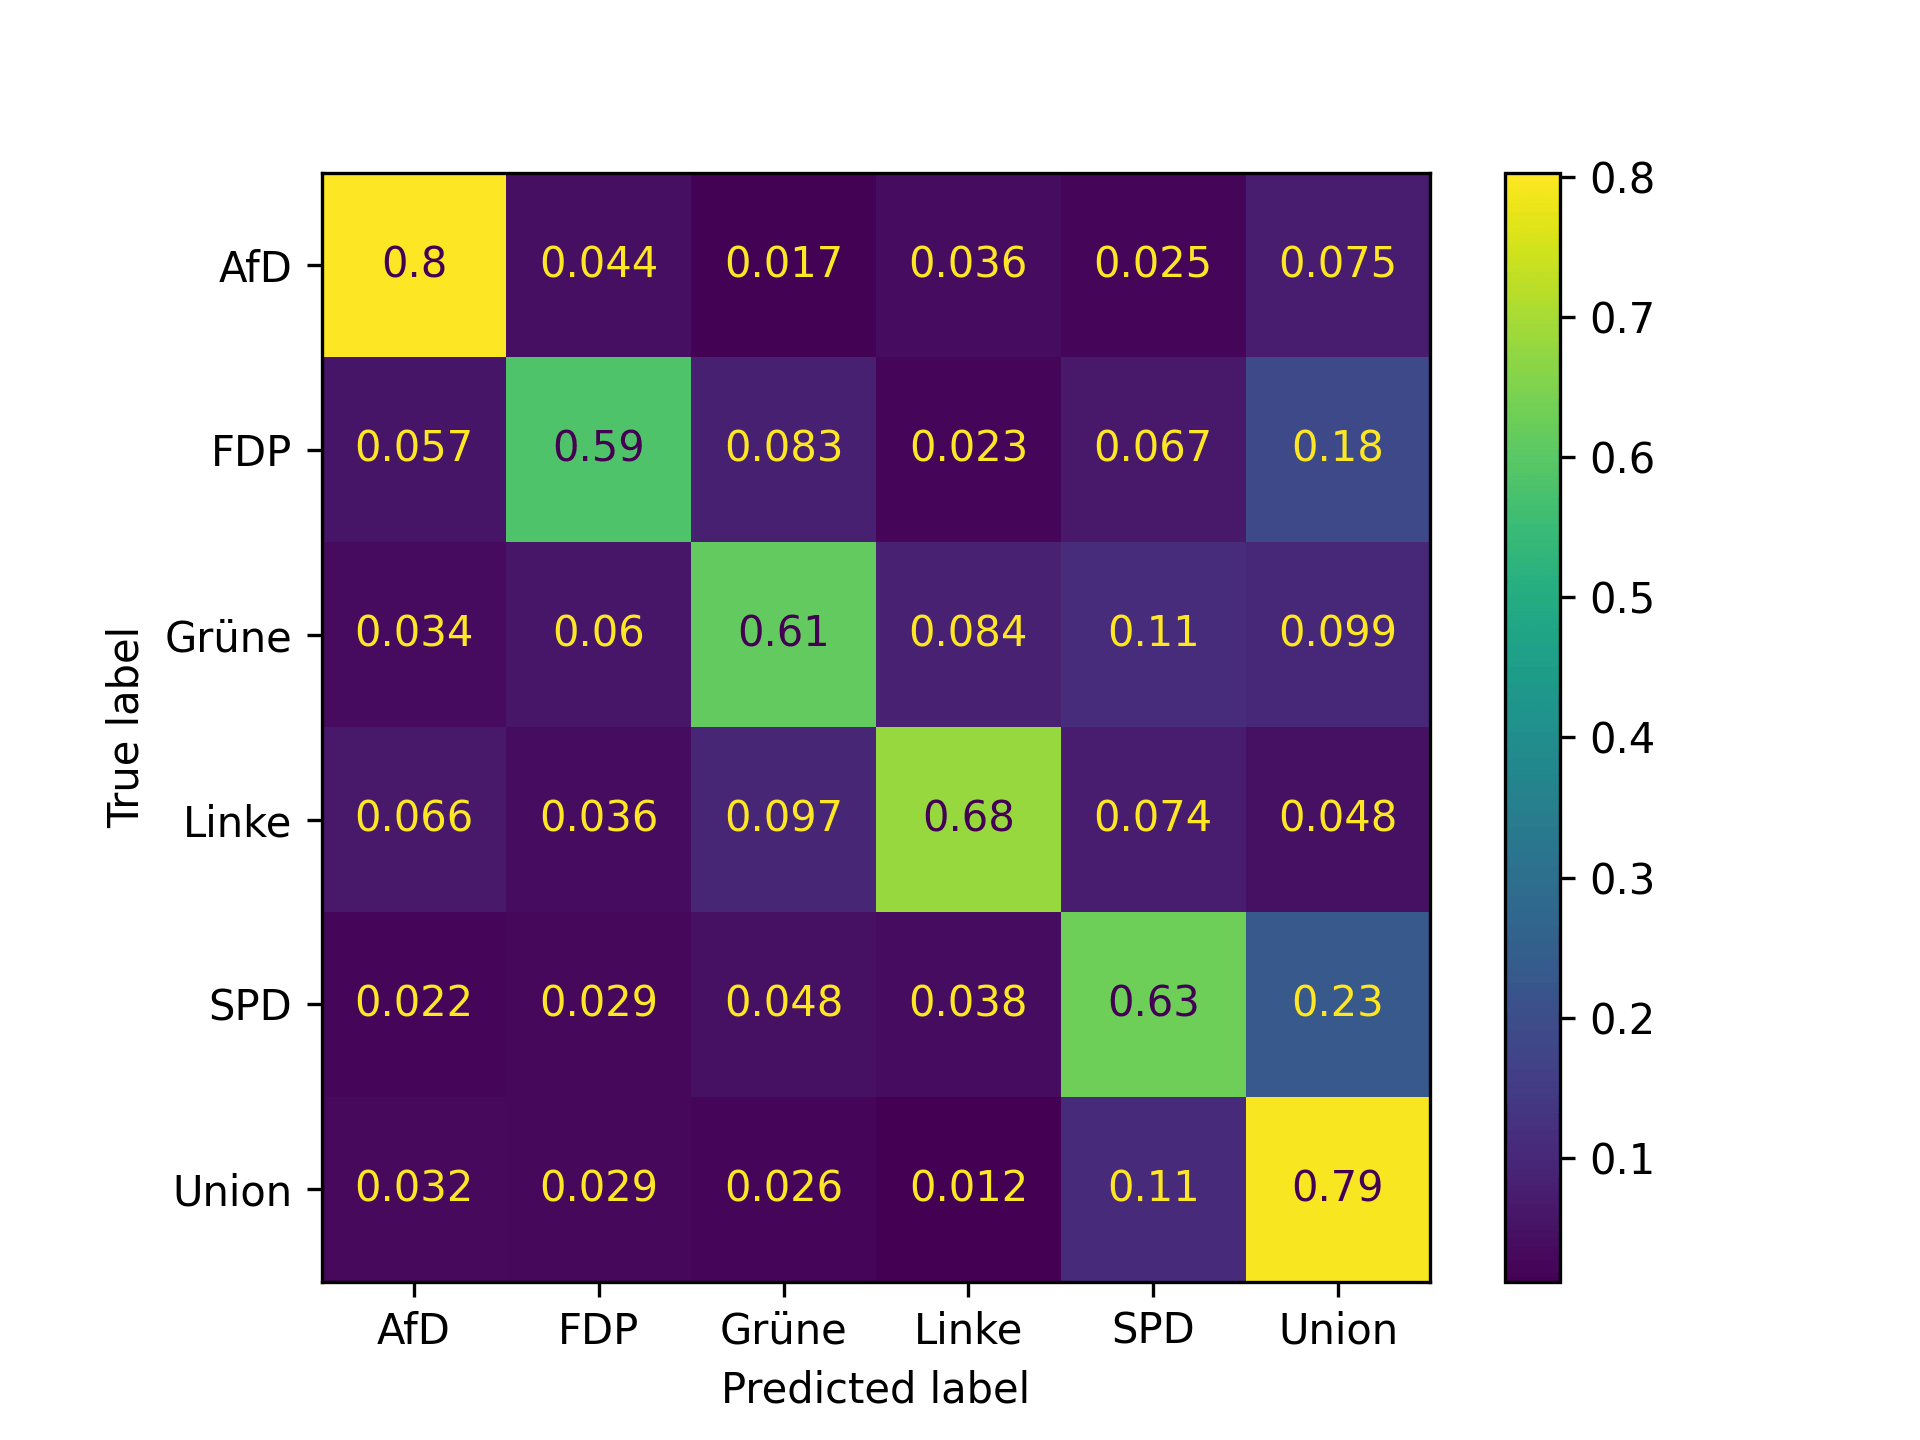
\includegraphics[width=0.9\textwidth]{data/images/modeling/fasttext/none/speeches_confusion_matrix.png}
      \caption{Reden (\(N = \num{38475}\))} \label{sfig:confusionMatrixFastTextSpeechesUnbalanced}
    \end{subfigure}
    \hfill
    \begin{subfigure}{0.49\textwidth}
      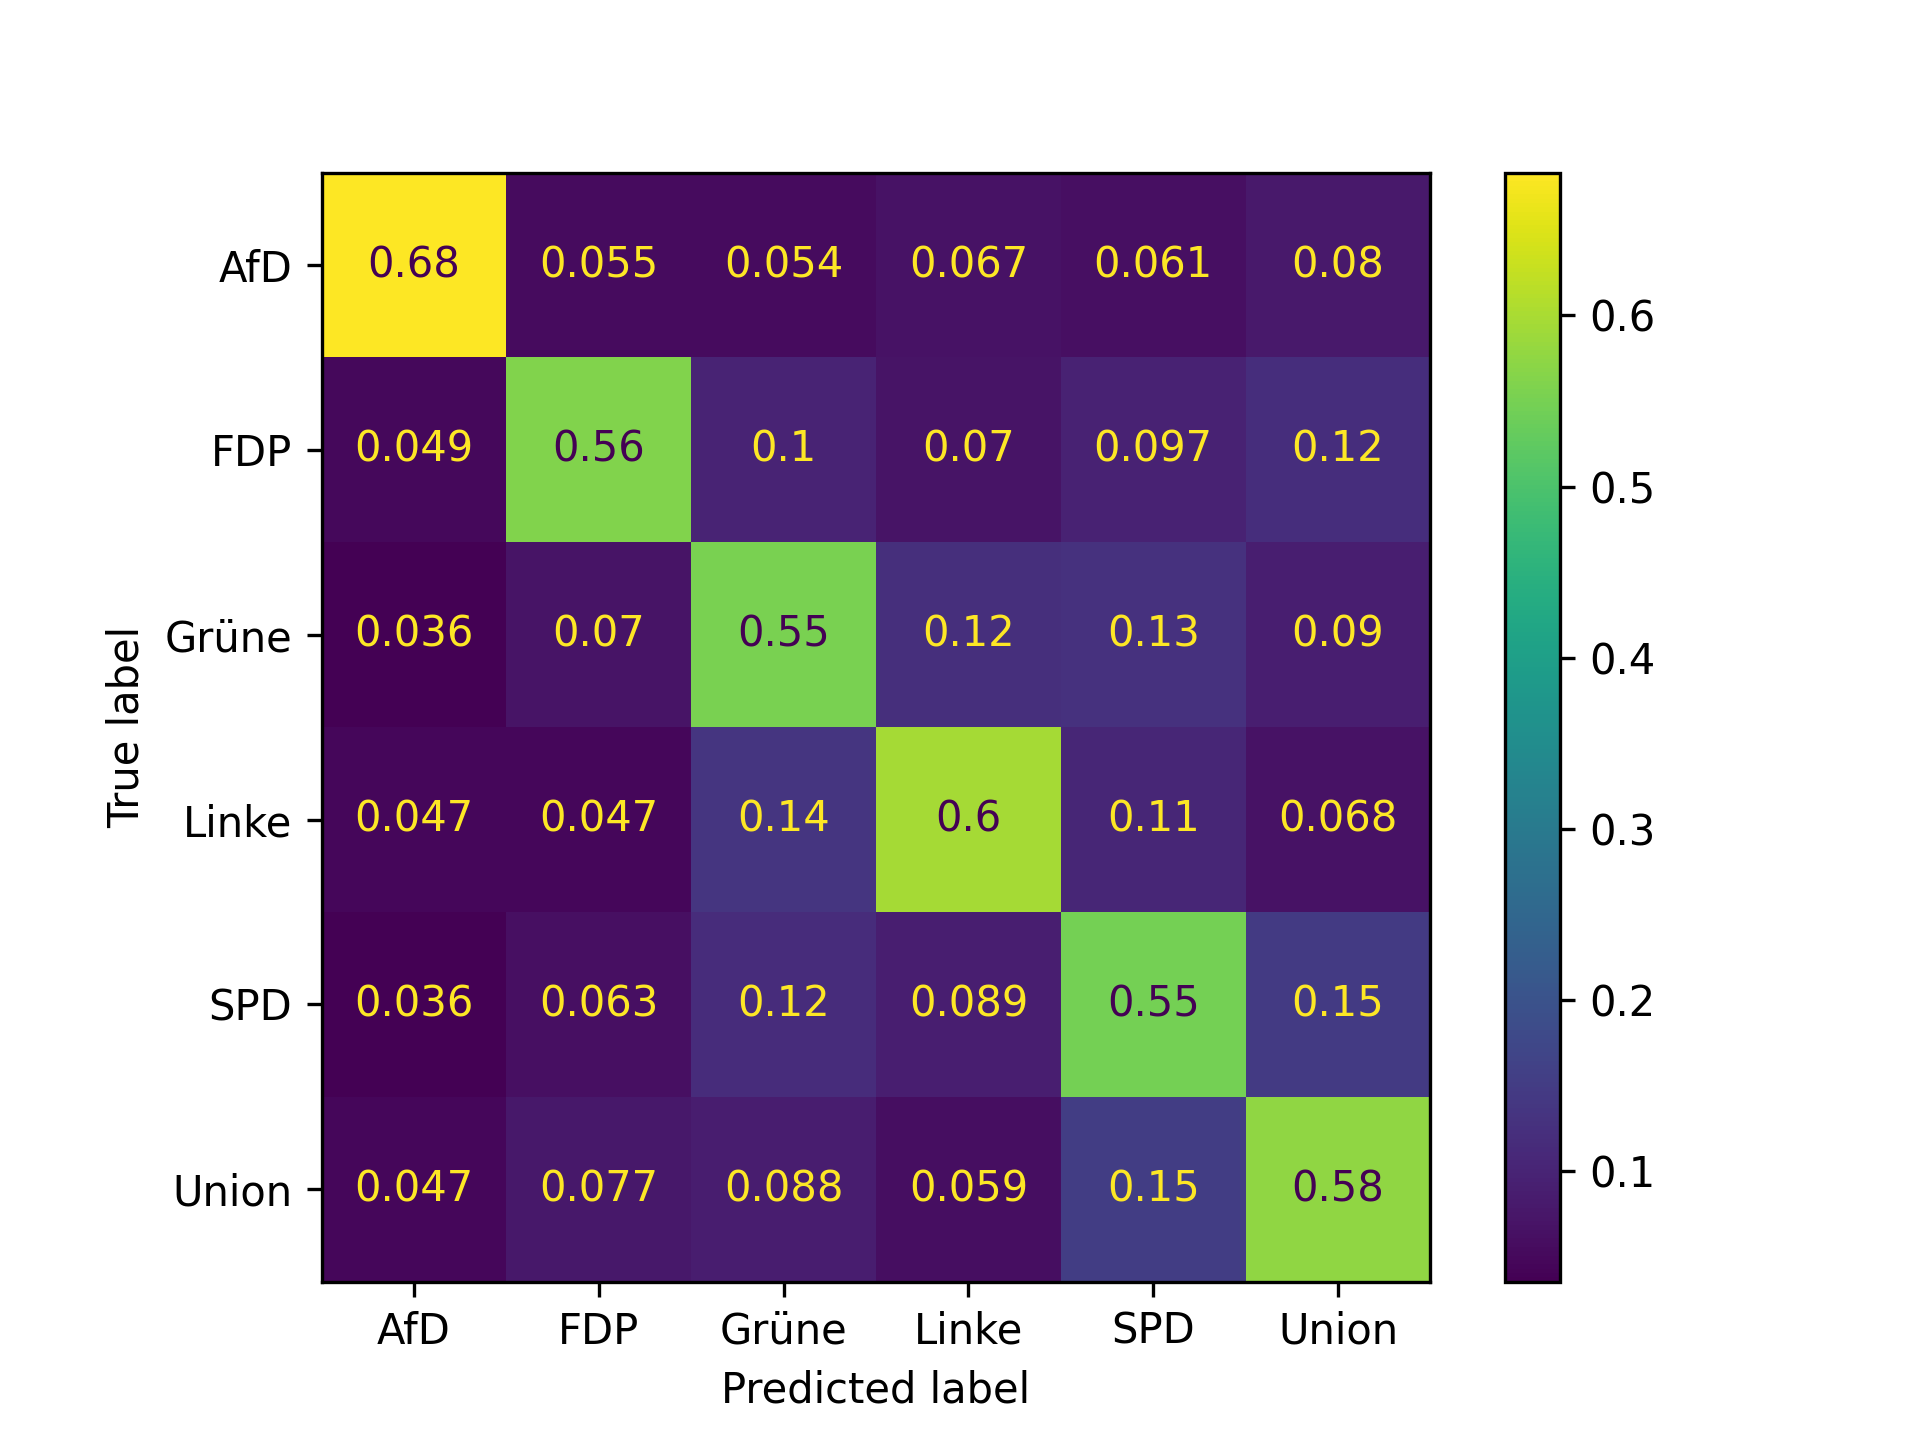
\includegraphics[width=\textwidth]{data/images/modeling/fasttext/none/all_confusion_matrix.png}
      \caption{Kombiniert (\(N = \num{392774}\))} \label{sfig:confusionMatrixFastTextAllUnbalanced}
    \end{subfigure}
    \caption[Konfusionsmatrizen für \ft mit Bigrammen (\(n = \num{2}\)) auf unausgeglichenen Datensätzen]{Konfusionsmatrizen für \ft mit Bigrammen (\(n = \num{2}\)) auf unausgeglichenen Datensätzen. \(N\) repräsentiert die summierte Anzahl an Trainings- und Testdaten.} \label{fig:unbalancedConfusionMatrixFastText}
\end{figure}

\subsection*{Multi-Layer Perceptron}

% TODO

\subsection*{CNN}

% TODO

\subsection*{BERT}

% TODO
